\documentclass[oneside]{article}


\usepackage{textcomp}
%change font. (ALTERNATIVE:  mathpazo, mathptmx, helvet, avant, courier, chancery, bookman, newcent, charter)
\usepackage{charter} % math & rm 
\normalfont
\renewcommand{\ttdefault}{lmtt} %tt

\usepackage[utf8]{inputenc}
\usepackage[italian]{babel}
\usepackage[T1]{fontenc} % Use 8-bit encoding that has 256 glyphs
%\usepackage[latin3]{inputenc}
%\linespread{1.05} % Line spacing - Palatino needs more space between lines
\usepackage{microtype} % Slightly tweak font spacing for aesthetics
\usepackage[hmarginratio=1:1,top=32mm,columnsep=20pt]{geometry} % Document margins
\usepackage{multicol} % Used for the two-column layout of the document
\usepackage[hang, small,labelfont=bf,up,textfont=it,up]{caption} % Custom captions under/above floats in tables or figures
\usepackage{booktabs} % Horizontal rules in tables
\usepackage{float} % Required for tables and figures in the multi-column environment - they need to be placed in specific locations with the [H] (e.g. \begin{table}[H])
\usepackage{hyperref} % For hyperlinks in the PDF
\usepackage{lettrine} % The lettrine is the first enlarged letter at the beginning of the text
\usepackage{paralist} % Used for the compactitem environment which makes bullet points with less space between them
\usepackage{lipsum} % Package to generate dummy text throughout this template
\usepackage{graphicx}
%abstract
\usepackage{abstract} % Allows abstract customization
\renewcommand{\abstractnamefont}{\normalfont\bfseries} 
\renewcommand{\abstracttextfont}{\normalfont\small} 

%titolo
\usepackage{titlesec} 
\renewcommand\thesection{\Roman{section}}
\renewcommand\thesubsection{\Roman{subsection}} 
\titleformat{\section}[block]{\Large\bfseries\scshape\centering}{\thesection.}{1em}{} 
\titleformat{\subsection}[block]{\large\scshape}{\thesubsection.}{1em}{} 
\titleformat{\subsubsection}[block]{\scshape}{\thesubsubsection.}{1em}{} 




%headers & footers 
\usepackage{fancyhdr} % Headers and footers
\pagestyle{fancy} % All pages have headers and footers
\fancyhead[L]{\bfseries{{\textsf{Davide Tedesco}}}}
\fancyhead[R]{\bfseries{{\textsf{$\bullet$ Verso una nuova frontiera della
 chitarra classica $\bullet$ }}}}
%\fancyhead[R]{\small \leftmark}
\cfoot{\thepage}




%----------------------------------------------------------------------------------------
%	TITLE SECTION
%----------------------------------------------------------------------------------------
\thispagestyle{empty}


\title{\vspace{-15mm}\fontsize{24pt}{10pt}\selectfont\textsf{\bfseries{\textsc{Verso una nuova frontiera della
 chitarra classica}}}} % Article title

\author{
\large
\textsc{Davide Tedesco}\\
\small \href{mailto:enter_adress_here}{\texttt{davide.tedesco.rome[at]gmail[dot]com}} 
%\vspace{-5mm}
}

\date{Luglio 2020}

%----------------------------------------------------------------------------------------




\begin{document}

\maketitle % Insert title

\tableofcontents

\thispagestyle{empty} 

%----------------------------------------------------------------------------------------
%	ABSTRACT
%----------------------------------------------------------------------------------------
\vspace*{10mm}

\begin{abstract}

%\noindent
La composizione per strumento solo è andata negli anni via via accrescendosi, sia per le possibilità donate dall'arte musicale elettronica, che per l'interesse degli esecutori allo sviluppo di un nuovo linguaggio oltre quello che corrisponde al repertorio. Questo atteggiamento è particolarmente visibile nell'ambiente compositivo chitarristico, nel quale non solo compositori di professione, ma gli strumentisti stessi si sono iniziati a porre la questione del come potesse esser interpretata la loro performance all'interno di un discorso contemporaneo. La chitarra, che di per se si presta a vari utilizzi, viene dunque paragonata spesso a soli gesti virtuosistici che non nutrono un vero senso compositivo alimentando un discorso compositivo che porta la qualità dei manufatti musicali sempre più verso la semplicità e immediatezza di esecuzione. Il compositore contemporaneo deve quindi osservare l'ambiente che lo circonda notando e annotandosi i punti forza attuali ed estendendo le possibilità (che un esecutore) gli propone, Il seguente testo mira dunque all'apertura ad una ricerca scientifico-compositiva che cerchi di donare nuovo splendore alla chitarra classica, facendo render conto all'esecutore l'ampio spettro di possibilità sonore di cui è in potere ed ampliandolo attraverso l'utilizzo di adeguati mezzi elettronici.

\vspace*{4mm}
\end{abstract}

\hspace*{4mm}

%----------------------------------------------------------------------------------------
%	ARTICLE CONTENTS
%----------------------------------------------------------------------------------------
\newpage
\begin{multicols*}{2} % Two-column layout throughout the main article text



%-----------------------------------------------------1= Introduzione
\section{ Introduzione}

La chitarra è forse lo strumento che nelle varie epoche più si è adattato e piegato al volere e alla necessità di chi lo adoprava, esso è stato allo stesso tempo un mezzo popolare e colto che ha subito cambiamenti costruttivi sostanziali, ma mantenendo sempre la massima manegevolezza. Se nell’ambito colto venne molto apprezzato nel 1600,l’800 e dalla metà del 1900, in ambito popolare è divenuto forse lo strumento per eccellenza nel Novecento ed è stato oggetto di un boom di vendite (ancora in atto) e di apprezzamento, grazie alla sua mutevole e sempre interessante predisposizione all’incoronazione di miti pop grazie al sua versione elettrica, acustica etc... Lo strumento originario oltre le sue possibilità di esecuzione per mezzo di eccitazione delle corde è stato negli anni studiato e re-interpretato e ne sono conseguiti sviluppi multipli. Da un lato l’ambito percussivo è stato esplorato con brani quali \textit{Ko-Tha} di Scelsi e dall’altro l’amplificazione dello strumento acustico ha reso possibile l’emersione di timbriche e sonorità non percepibili(ascolto del microcosmo timbrico), facendo sviluppare notevolmente il fenomeno del \textit{tapping}\footnote{Visionato dal pubblico italiano per la prima volta in uno storico video che ritrae Vittorio Camardese, medico di professione, ma esperto di tapping per hobby} e della ricerca sulla sola tastiera. Numerosi sono inoltre gli utilizzi e le possibilità donate dall’elettrificazione e dal radicale re-styling, che portati all’interno della musica colta come mezzi post-avanguardistici hanno dato luogo quasi ad una corrente della chitarra elettrica contemporanea con autori quali Romitelli\footnote{Trash TV Trance, 2002}  e Murail\footnote{Vampyr!, 1984}  ad esempio. 
La domande che sorgono da una prima panoramica sono: qual’è il ruolo della chitarra (classica, elettrica ed in tutte le sue versioni) nella musica contemporanea oggi? Essa è ancora uno strumento attuale? Quale deve essere l’atteggiamento del compositore verso uno strumento usato tanto per il suo repertorio popolare, quanto per il suo repertorio classico? Questo breve testo cerca di esplicare e trarre spunto ed approfondire alcuni aspetti portando la chitarra classica nel presente ed ripensando l’elettrificazione della stessa e la necessità di un’operazione del genere. 


%----------------------------------------------------2= La chitarra

\section{ La chitarra}

Dalla famiglia dei liuti nel 500 d.C. circa, si iniziarono ad intravedere alcune delle più moderne versioni dello strumento con il guscio (la cassa armonica) non più di forma tondeggiante, ma esso fu sostituito da due superfici piatte unite da una fascia.
\includegraphics[width=0.4\textwidth]{img/chit_spaccato.png}
Anche se l’origine della chitarra ci indica che essa provenga dal liuto, il tempo l’ha portata con sé fino ai giorni nostri, e questo strumento attraversando i secoli ha cambiato varie volte nome e già nel XIV secolo troviamo il nome di chitarra moresca in un libro spagnolo, che variando nome, venne chiamata in seguito mandola.
Questi strumenti a corda pizzicata attraverso un plettro od una penna ebbero spesso quattro corde a simboleggiare le quattro fasi della luna, le settimane del mese e via discorrendo, gli accordi, o in ogni caso il modo di suonare simultaneamente più corde era in quel periodo sconosciuto ai più, e lo strumento era suonato inizialmente solamente per eseguire una melodia ed occasionalmente vi venivano eseguiti degli ostinati per accompagnare questa melodia, con il passare dei secoli e dei luoghi in cui lo strumento fu portato e sviluppato, le sapienze orientali e occidentali si mescolarono fino a renderlo in Andalusia il liuto che conosciamo.
Il liuto divenne lo strumento predominante in Europa tra 1500 e 1700, anche se in quel periodo in Spagna non era molto apprezzato ed utilizzato dall’aristocrazia, la musica popolare spagnola fece invece conoscere la chitarra al resto d’Europa. Benché la musica colta veniva invece eseguita su di una vihuela, in genere la vihuela da mano, che si differenziava dalla vihuela da arco per il modo in cui la si suonava, la vihuela da mano aveva 6 o 7 corde ed era accordata in vari modi.
L’arte liutistica ebbe il suo declino verso la fine del ‘600 quando strumenti come il clavicembalo molti altri strumenti a tastiera iniziarono a prendere piede, ma con il declino del liuto la  chitarra inizió ad essere più apprezzata, soprattutto per la sua maneggevolezza e facilità di trasporto.
Sui principi del 600 la chitarra aveva solamente quattro corde doppie, che erano accordate spesso  “Do-Fa-La-Re” o “Fa-Si-Re-Sol”. 
In questo periodo la chitarra aveva la cassa armonica più stretta e profonda.
La chitarra italo-spagnola incominciò a viaggiare in Europa arrivando prima di tutto all’aristocrazia francese, e venne raffigurata più e più volte in affreschi alla corte francese.
La chitarra divenne dunque uno strumento da dilettanti e fu semplificata, sei corde singole e non più doppie con accordatura “Mi-La-Re-Sol-Si-Mi”, ovvero l’accordatura tradizionale che abbiamo ancora oggi.
Il nuovo modello di chitarra era dunque maturo e divenne più facile da maneggiare. Nell’800 venne poi introdotta un’altra miglioria con la sostituzione dei piroli in legno con quelli a viti in metallo.
La chitarra ebbe alti e bassi nella sua diffusione e per il suo gradimento generale e furono divisi fino al  primo ‘900 per ambito colto e popolare.
Essa fu riportata, in ambito colto, a dei livelli altissimi grazie all’apporto di figure come Andrés Segovia, Joaquin Rodrigo e Heitor Villa-Lobos.


%----------------------------------------------------3= La chitarra nella musica contemporanea

\section{ La chitarra nella musica contemporanea}

Iniziando a scavare all'interno della storia della composizione per questo strumento, non si puó far altro che passare per i classici oramai intramontabili che ogni studente di Conservatorio incontra ed oltre ai già nominati Segovia, Rodrigo e Villa-Lobos, ci si ritrova ad osservare scaffali interi dei negozi in cui si sono inseriti centinaia di studi per chitarra di autori quali: Sor, Giuliani, Carulli e via dicendo. Non dobbiamo dunque stupirci al fatto che in sede di concerto il chitarrista tenda a realizzare una gara \textit{all'esecuzione piú veloce}, poichè la premessa didattica è sempre stata improntata alla ricerca della velocità di esecuzione ed alla perfezionamento del virtuosismo. Laddove invece si trovano degli esecutori in grado di interpretare e contestualizzare un'opera si trovano invece delle gemme, che riescono veramente a far prender forma alle composizioni per chitarra sola. Ne sono esempi Elena Casoli\footnote{}, Arturo Tallini\footnote{} e Ruben Mattia Santorsa\footnote{}, oltre a molti altri nel panorama internazionale, che attraverso la collaborazione proficua con compositori, alunni e conservatori riescono a delineare dei progetti dal piú vasto respiro ed a donare uno spazio per la chitarra all'interno della \textit{giungla} musicale odierna.
%\begin{figure}
\includegraphics[width=0.5\textwidth]{img/ektopos.png}
%\caption{Agostino Di Scipio - Ektopos}
%\label{img/ektopos.png}}
%\end{figure}
L'ambiente chitarristico rivela dunque alcune dei suoi gioielli proprio attraverso degli esecutori che sono riusciti a comprendere il ruolo che il proprio strumento può avere e ponendosi con occhio ed orecchio vigile allo studio delle partiture contemporanee. Se da un lato ci si aspetterebbe un vasto repertorio chitarristico contemporaneo ricco di idee e nuove possibilità, da un certo punto di vista si rimane delusi, trovando opere realizzate da grandi e rinomati compositori quali Berio\footnote{}, Ferneyhough\footnote{} e Maderna\footnote{}, 
che rispecchiano però un'idea di composizione \textit{novecentesca}. Si trovano invece spunti di riflessione brillanti in compositori a noi piú vicini come Di Scipio\footnote{Ektopos, in figura}, Murail\footnote{Tellur} e Romitelli\footnote{Solare, Seascape ed altre opere}. Sebbene queste composizioni riescano in ogni modo a dar giustizia alle sei corde, troviamo nel brano di Scelsi \textit{Ko-Tha}\footnote{del 1962} una piú vasta ricerca sul suono ed una prima esperienza chitarristica percussiva che cerca di sfruttare lo strumento in maniera non convenzionale. Dall'ascolto delle registrazioni \textit{scelsiane} custodite alla \textit{Fondazione Isabella Scelsi} notiamo dunque una vera e propria ricerca del e sul suono che si avvicina al microcosmo timbrico piú di quanto altri compositori dopo di lui sono riusciti a fare. Dunque l'utilizzo dello strumento come una percussione, degli strappati e delle possibilità al di fuori del melodico iniziano veramente a ristrutturare la concezione compositiva dello strumento. La ricerca e la risposta di Berio è invece (come in tutte le sue sequenze) una \textit{creazione di un virtuosismo} che punta al far esperire lo strumento e le sue capacità melodico-armoniche al massimo delle sue possibilità. 
Se dunque l'utilizzo della chitarra classica all'interno dell'ambito contemporaneo riesce in qualche modo a tagliare la tela della tradizione, le esperienze menzionate in precedenza di interventi musicali con la chitarra elettrica, entrano possentemente all'interno del paesaggio musicale, rendendo ben visibili le possibilità timbriche, compositive e teatrali che uno strumento popolare quanto diffuso puó realizzare. Non è un caso che le composizioni per chitarra elettrica di Murail e Romitelli siano costantemente suonate, proposte e pubblicate sul web. 
Se dunque questo lo strumento \textit{rivisitato} è riuscito a portare tanta novità e apprezzamento, perchè la chitarra classica rimane sempre piú nell'ombra del panorama colto?
L'utilizzo dell'elettronica all'interno del panorama musicale tradizionale per strumento solo è come se sia vista come un di piú, da poter incollare accanto o come sfondo al suono dello strumento solo, rendendo di fatto pochissime composizioni per chitarra classica ed elettronica sensate.

%----------------------------------------------------4= L’aumentazione: l'amplificazione, Il feedback e la distorsione

\section{ L’aumentazione: l'amplificazione, Il feedback e la distorsione}

In questo vasto ambiante compositivo ed esecutivo che porta con se brillantezza e freschezza di idee, vi è però sempre dunque un minimo comun denominatore, ovvero lo strumento solo rilegato alle sue possibilità strutturali oramai trite e ritrite. Forse si puó notare nella mancanza dell'elettronica all'interno del discorso compositivo chitarristico classico, una voglia di legame con il passato che sta portando a lungo andare alla dispersione dei risultati raggiunto nel '900, lasciando lo strumento in mano alla sola musica popolare. 

\noindent Da queste riflessioni nasce dunque la necessità di provare a realizzare un qualcosa che potesse integrare l'elettronica con lo strumento, come è già stato fatto per molti altri strumenti soli, riuscendo a captare il microscopico dello strumento, le caratterizzazioni fisiche dello strumento e le possibilità donate dall'esperienza della chitarra elettrica nel contemporaneo.
\noindent
\newline
\textbf{Amplificazione} \newline
\textbf{Feedback} \newline
\textbf{Distorsione} \newline

video esempio gestione del feedback\footnote{https://www.youtube.com/watch?v=7BwwTopM3Ek}
video esempio Distorsione\footnote{https://www.youtube.com/watch?v=K3yqyxcJStg}
\includegraphics[width=0.5\textwidth]{img/ir.png}
\includegraphics[width=0.3\textwidth]{img/guitarLive.png}


%----------------------------------------------------5= Gli sketches e gli studi per chitarra
\section{ Gli sketches e gli studi per chitarra}

Alla ricerca non di un nuovo strumento, ma bensí di un nuovo linguaggio e di una ricerca di un virtuosismo non basato sulla sola velocità dell’esecuzione dei brani, il compositore osservando il contemporaneo ed estrapolando la sua idea deve tentare di riportarlo sullo strumento.
\includegraphics[width=0.5\textwidth]{img/luoghi_perc.png}

%----------------------------------------------------6= Conclusioni

\section{ Conclusioni}

Dal lavoro di ricerca effettuato sorgono, oltre a notevoli ed importanti traguardi per la composizione chitarristica, delle perplessità. Nell’utilizzo di uno strumento come la chitarra la standardizzazione della costruzione dello strumento è sempre stato un qualcosa che i costruttori non hanno voluto attuare, rendendo di fatto totalmente diverse le costruzioni e le caratteristiche interne dello stesso.
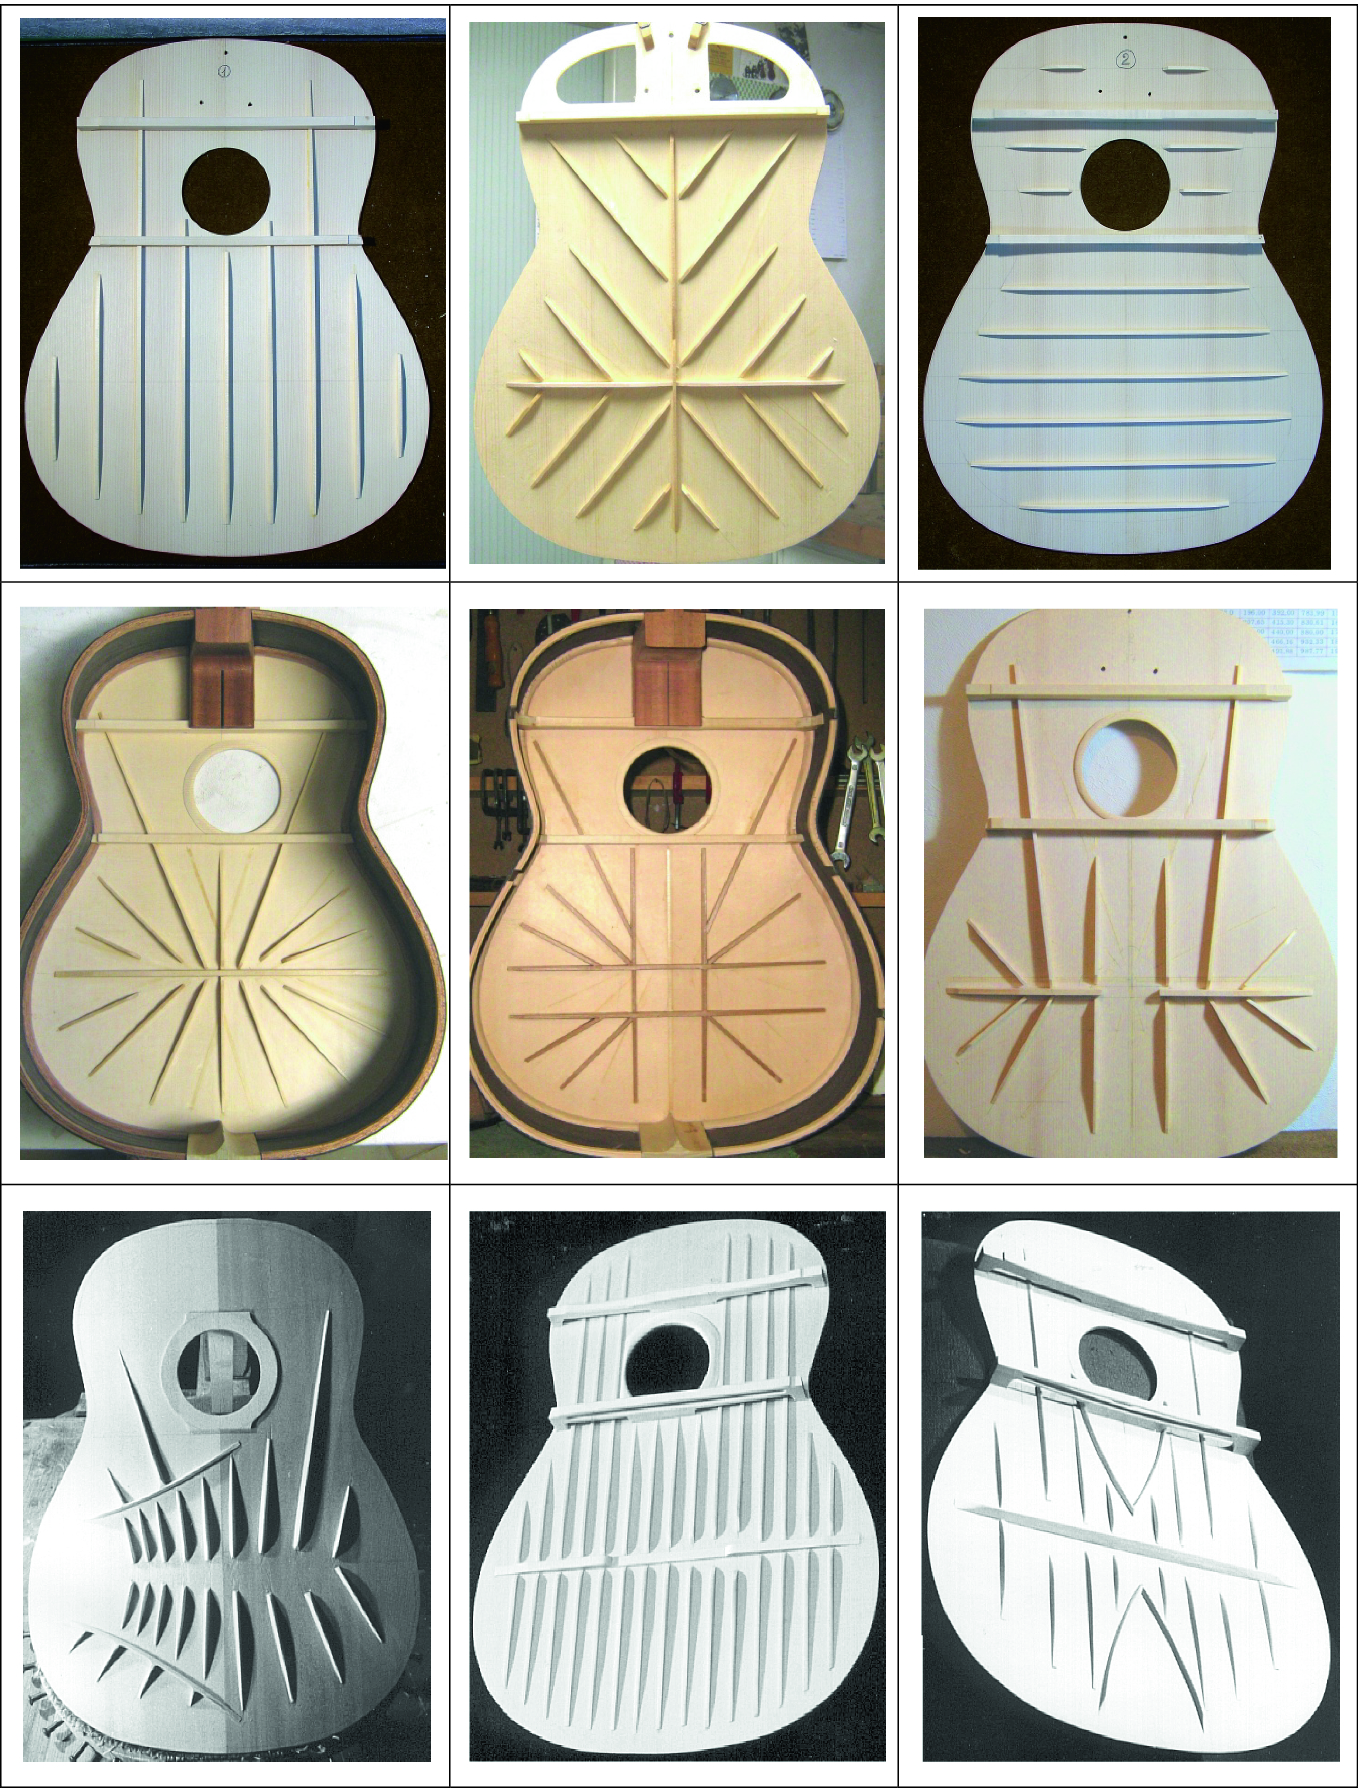
\includegraphics[width=0.5\textwidth]{img/catene.png}
La ricerca effettuata fin qui è stata eseguita infatti su di una chitarra che presenta le catene\footnote{parte interna chitarra} realizzate in un certo modo che fanno si che essa abbia una particolare risposta all’eccitazioni proposte.
\includegraphics[width=0.5\textwidth]{img/chladni1.png}
I patterns di Chladni  di una chitarra possono ad esempio farci intendere quali siano i punti nodali dello strumento aiutandoci nel posizionamento di un sensore piezo-elettrico o di un attuatore sul piano armonico, ma ogni strumento avrà dei suoi punti che faranno espletare al meglio risultati analoghi. Bisogna quindi precisare che la ricerca in questa direzione cercando di sfruttare lo strumento nel miglior modo possibile dovrà esser seguita dal compositore e che egli dovrà fornire degli strumenti adeguati per far preparare lo strumentista all'esecuzione in concerto. Questi strumenti saranno un vero è proprio mezzo che dovrà accompagnare nella messa in scena musicale e dovranno preparare lo strumento all'esecuzione. Si punta quindi ad una ricerca da parte dello strumentista che possa far trasparire l'intenzione compositiva anche attraverso strumenti realizzati costruttivamente in maniere differenti.
La ricerca di un metodo chiaro di scrittura è inoltre un altro punto fondamentale, esso chiarirà ogni dubbio dell'esecutore ogni qualvolta 

Il seguente testo è a corredo dal materiale elaborato, studiato ed approfondito durante il corso dell'anno reperibile attraverso il link al piè.\footnote{https://github.com/SMERM/BN-Tedesco/tree/master/COME-02}

\newpage
%===============================================Sitografia & bibliografia

\section{ Bibliografia \& sitografia}
•\textsc{\textsf {Arturo Tallini}}, \emph{MusicaIncerta, un'introduzione alla musica contemporanea per chitarra}, UT Orpheus 2000\\
•\textsc{\textsf {Arturo Tallini}}, \emph{Ma! con note scritte}, Editor 2000\\
•\textsc{\textsf {Curt Sachs}}, \emph{Storia degli strumenti musicali}, Mondadori 1980\\
•\textsc{\textsf {Emilio Pujol}}, \emph{El dilemmma del sonido en la guitarra}, Ricordi 1979\\
•\textsc{\textsf {Carlo Carfagna, Michele Greci}}, \emph{Chitarra, storia e immagini}, Fratelli Palombi Editori 2000\\
•\textsc{\textsf {Rita Torres, Paulo Ferreira-Lopes}}, \emph{Towards Overcoming the Guitar's Color Research Gap}, CITAR 2014\\
•\textsc{\textsf {Jonathan Godfrey}}, \emph{Principles of Idiomatic Guitar Writing},  2013\\
•\textsc{\textsf {John Schneider}}, \emph{The Contemporary Guitar},  University of California Press 1985\\

\hspace*{10mm}

%===============================================Brani ascoltati e partiture visionate

\section{ Brani ascoltati \& partiture visionate}
•\textsc{\textsf {Agostino Di Scipio}}, \emph{Ektopos}, UT Orpheus 2000\\
•\textsc{\textsf {Azio Corghi}}, \emph{Consonancias y Redobles}, Universal Edition 1973\\
•\textsc{\textsf {Barbara Kolb}}, \emph{ - Looking for Claudio}, Boosey \& Hawkes 1975\\
•\textsc{\textsf {Benjamin Britten}}, \emph{Nocturnal After John Dowland}, xx 199x\\
•\textsc{\textsf {Brian Ferneyhough}}, \emph{Kurze Schatten II}, xx 199x\\
•\textsc{\textsf {Brian Ferneyhough}}, \emph{no time}, xx 199x\\
•\textsc{\textsf {Bruno Maderna}}, \emph{Y Después}, xx 199x\\
•\textsc{\textsf {Bruno Maderna}}, \emph{Serenata per un satellite}, Ricordi 1969\\
•\textsc{\textsf {Fabio Vacchi}}, \emph{Plynn}, xx 199x\\
•\textsc{\textsf {Fabrizio Casti}}, \emph{ L' 'Anima Visionaria}, UT Orpheus 2000\\
•\textsc{\textsf {Fausto Romitelli}}, \emph{Trash TV Trance}, Ricordi 2002\\
•\textsc{\textsf {Fausto Romitelli}}, \emph{Solare}, Ricordi 1984\\
•\textsc{\textsf {Fausto Romitelli}}, \emph{La lune et les eaux}, Ricordi 1991\\
•\textsc{\textsf {Fausto Romitelli}}, \emph{Seascape}, Ricordi 1994\\
•\textsc{\textsf {Fausto Romitelli}}, \emph{Coralli}, Ricordi 1987\\
•\textsc{\textsf {Fausto Romitelli}}, \emph{Highway to hell}, Ricordi 1984\\
•\textsc{\textsf {Franco Donatoni}}, \emph{Algo}, xx 199x\\
•\textsc{\textsf {Giacinto Scelsi}}, \emph{Ko-Tha}, Salabert 1962\\
•\textsc{\textsf {Helmut Lachenmann}}, \emph{Salut für Caudwell}, xx 199x\\
•\textsc{\textsf {Luciano Berio}}, \emph{Sequenza XI}, Universal Edition 1988\\
•\textsc{\textsf {Maurizio Pisati}}, \emph{Set7}, Kairos 2017\\
•\textsc{\textsf {Sylvano Bussotti}}, \emph{Ultima rara,}, xx 1969\
•\textsc{\textsf {Tristan Murail}}, \emph{Tellur}, xx 1977\\
•\textsc{\textsf {Tristan Murail}}, \emph{Vampyr!}, xx 199x\\
•\textsc{\textsf {Toru Takemitsu}}, \emph{12 songs for guitar}, Schott 2005\\
•\textsc{\textsf {Toru Takemitsu}}, \emph{All In Twilight}, Schott 1993\\
•\textsc{\textsf {Toru Takemitsu}}, \emph{Equinox}, Schott 1993\\
•\textsc{\textsf {Toru Takemitsu}}, \emph{To the edge of dream}, xx 199x\\


\end{multicols*}

\end{document}
